\section{The Radio Access Network}\label{sec:RAN}

\begin{figure*}[ht]
 \begin{center}
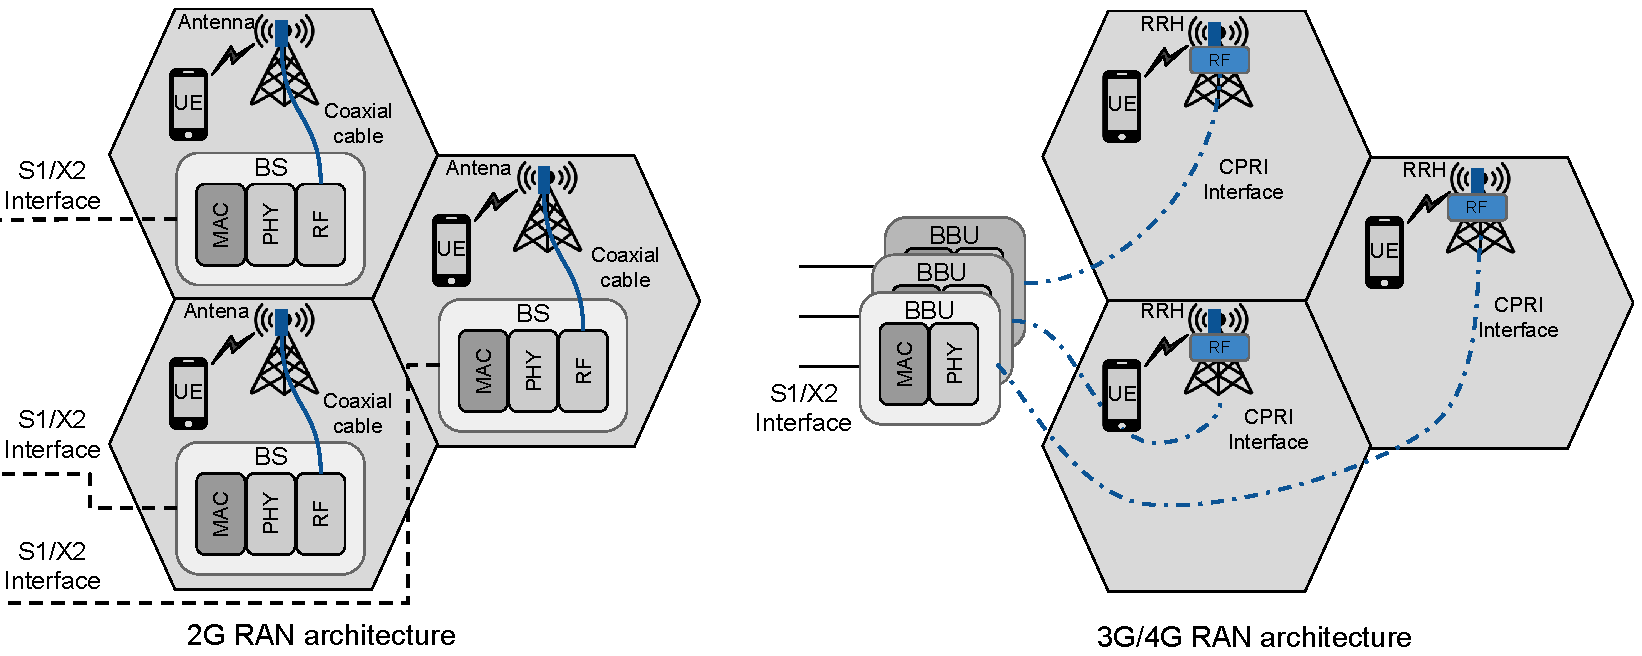
\includegraphics[width=0.8\textwidth]{figs/EvolucaoRAN_1.pdf}
  \end{center}
\caption{Evolution of RAN architectures.}
\label{fig:evolucaoRAN}
\end{figure*}

A RAN is responsible for managing the air interface to keep a large number of users connected. Therefore, RAN needs to efficiently manage the RF spectrum, performing a series of tasks, such as radio resource management, connection mobility control, dynamic allocation of resources to users' equipment, compression and security in the physical layer, session management, and QoS flow, among other functions.

Initially, on a traditional RAN, the RF front-end and baseband processing functionalities were integrated within a BS. The antenna module was located a few meters from the radio module, connected with a coaxial cable, and showed high transmission losses. This architecture was noted on 1G and 2G mobile networks. In recent years, the RF front-end has been decoupled from the baseband processing module, allowing mobile operators to replace this module according to user demand. This architectural decoupling allowed advances in centralization and virtualization in the baseband processing module and the RF front-end. Next, Subsection \ref{subsec:CRAN} presents the evolution of the concept of centralization of baseband architecture, and Subsection \ref{subsec:VRAN} presents the virtualization of RAN, which started in 4G and continues to evolve in networks 5G.


\subsection{RAN centralization} \label{subsec:CRAN}

The high data transmission rate between the digital baseband processing domain and the analog domain of the RF front-end with the antenna requires a high bandwidth bus that connects these two domains. For many years, this requirement has limited the BS design to specialized hardware components with that high-performance bus. This limitation was overcome with the use of fiber optics on this bus, reducing data loss and increasing the distance between the connected domains. In 3G/4G generations, especially since Release 8 of the 3GPP, the baseband processing started to be implemented in BBUs, \textit{i.e.}, dedicated and specialized hardware that implements a RAT. At the same time, RRH integrates the RF front-end with the antenna. In Fig.~\ref{fig:evolucaoRAN}, the evolution of the RAN architecture from 2G to 3G/4G is illustrated.

In 3G/4G, the RF front-end and the baseband processing are separated, as can be seen on the right side of Fig.~\ref{fig:evolucaoRAN}. RRH also called a Radio Unit (RU), has a fiber optic interface and performs analog/digital conversion and vice-versa, power amplification, and signal filtering. The baseband processing, now performed at BBU, is isolated and independent from RU. This architecture is considered decentralized since BBU performs its operation separately from RU. Recent advances have boosted the bandwidth of optical fibers allowing the incorporation of cloud-based architectures into the Cloud Radio Access Network (C-RAN). In this type of architecture, BBUs can be located in a data center (called centralized baseband architectures), allowing cost reduction through centralized maintenance and by the elasticity of cloud computing. In this new configuration, RRHs can be geographically separated from a set of BBUs by up to approximately 40~km. However, it is important to note that a BBU is limited to processing RRH signals within a maximum distance, determined according to the delay restrictions. This delay is mainly influenced by three factors: (\textit{i}) distance between BBU and RRH, (\textit{ii}) channel conditions, and (\textit{iii}) available processing capacity. According to Marotta et al. \cite{Marotta:18}, the processing capacity should be increased significantly for RRHs that are experiencing low Signal-to-Noise Ratio (SNR) and long distance from the BBU. 

The concepts involved in C-RAN have been drawn attention to the initial implementation of 5G (Architecture NSA described in Subsection~\ref{sec:NSA}), mainly considering the benefits of cost reduction and maintenance. However, BBUs are hardware-based platforms using specialized digital signal processors. Including a long-term objective, it is essential to replace BBUs based on specialized hardware with software using general-purpose hardware, \textit{i.e.}, Virtual BBUs (vBBUs). In the same way, we can think of a radio virtualization layer that allows several heterogeneous access technologies coexisting on the same RRH. This coexistence uses innovative baseband processing techniques to divide and abstract an RRH into multiple virtual RRHs (vRRHs).  This vision of RAN virtualization is aligned with the SA Architecture (described in Subsection~\ref{sec:SA}) proposed in Release 15 of 3GPP, where, for example, the use of vBBUs is an Network Functions Virtualization (NFV) use case to provide services on a 5G system.


\subsection{RAN virtualization} \label{subsec:VRAN}

The RAN virtualization (vRAN) has received prominence in 5G systems because it allows us to create, manage, and configure RANs dynamically, meeting specific requirements of each service. Furthermore, the vRAN concept opens up new business models in which service providers can rent vRANs from infrastructure providers. In this scenario, the infrastructure provider controls the entire physical resource, including the RF spectrum, the physical RRH, the hardware resources in the data centers (\textit{i.e.}, servers with processing, memory, and storage) and the physical network. A service provider can hire from one infrastructure provider one or more vRANs, including at least one virtual BS, \textit{i.e.}, a vRRH connected to a vBBU.

\begin{figure*}[htb]
 \begin{center}
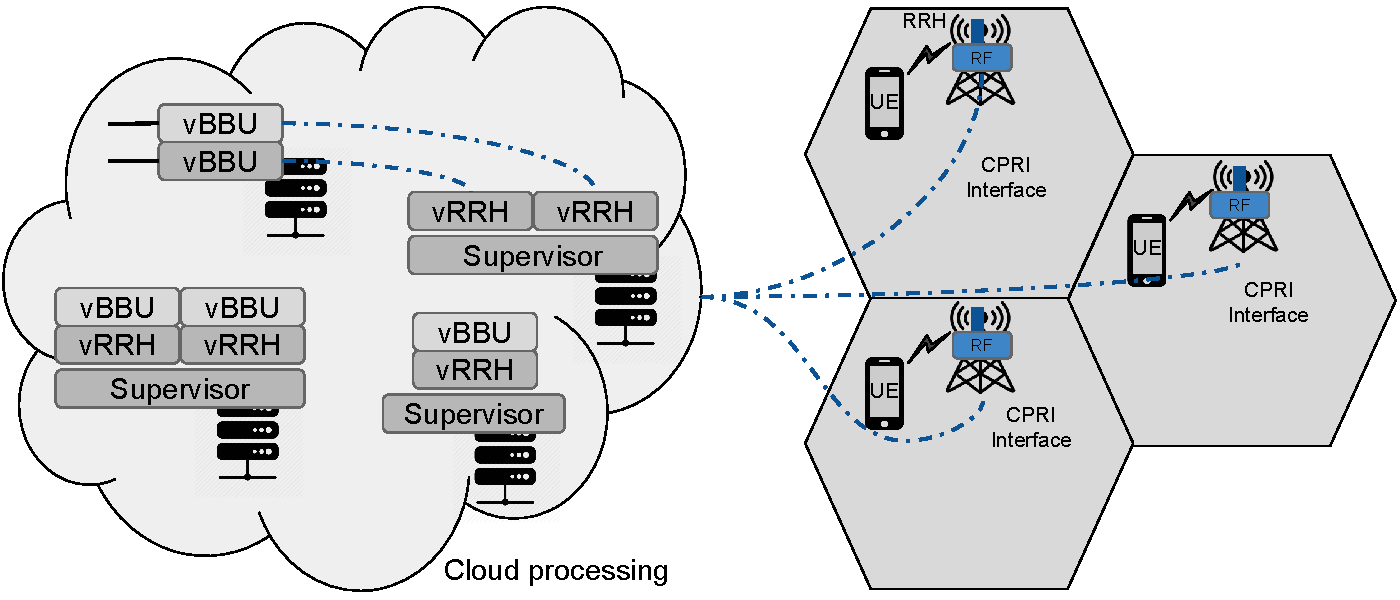
\includegraphics[width=0.7\textwidth]{figs/EvolucaoRAN_2.pdf}
  \end{center}
\caption{Virtualized RAN.}
\label{fig:vRAN}
\end{figure*}

Isolation, programmability, and adaptability are essential properties for customizing vRAN to accommodate the different services provided for 5G networks. For example, the combination of BBU and RRH slicing can instantiate an end-to-end vRAN over physical infrastructure. More specifically, slicing and virtualization can be implemented in a BBU to allow multiple vBBUs to run on the same physical hardware. Likewise, one RRH or a combination of them can support multiple vRRHs. These elements applied to vRAN, constitute the pillars to provide multi-services for future mobile networks.

A set of vBBU and vRRHs can be run on General Purpose Processor (GPPs), taking advantage of the highly optimized signal processing libraries and taking advantage of the ever-increasing evolution of processors, such as higher processing power and energy efficiency, such as can be seen in Fig. \ref{fig:vRAN}. Recently, the 3GPP RAN3 working group \cite{3gpp:TR38.801} considered dividing a vBBU into two new entities, named Data Unit (DU) and Control Unit (CU). DU can host time-limited physical layer functions, while CU hosts non-critical function resources, such as the MAC layer and higher control services. DU implementation is expected to cover an area of 10 to 20 km in radius, while CU implementation should cover areas from 100 to 200 km.

In Release 15 of 3GPP, the cloud concept was maintained in the RAN, but the name was changed to NG-RAN using an interface called NG. Due to interoperability between 4G and 5G, DU and CU have been renamed gNB-DU and gNB-CU, respectively. A gNB is responsible for some tasks, such as radio resource management, connection mobility control, dynamic allocation of resources to users' equipment, physical layer compression and security, session management, and QoS flow, among other functions. Therefore, the gNB protocol stack is detailed, considering PHY, MAC, RLC, PDCP, RRC, etc.

Virtualization also introduced the possibility of dividing the gNB protocol stack into network functions. In this context, 3GPP proposed eight options for the functional division between centralized and distributed units \cite{3gpp:TR38.801}, considering transport requirements, in particular flow and latency. González-Día et al. ~\cite{Gonzalez-Diaz:19} evaluated, in an experimental setting, three slicing options for fronthaul, in addition to an option for the DU backhaul, as illustrated in Fig.~\ref{fig:splitsLayers}. These eight slicing options proposed by 3GPP are still the subject of research ~\cite{fonseca-sbrc-2019} and development by academia and industry, as requirements for virtualization, processing, and functionality still need to be investigated.

\begin{figure}[htb]
 \begin{center}
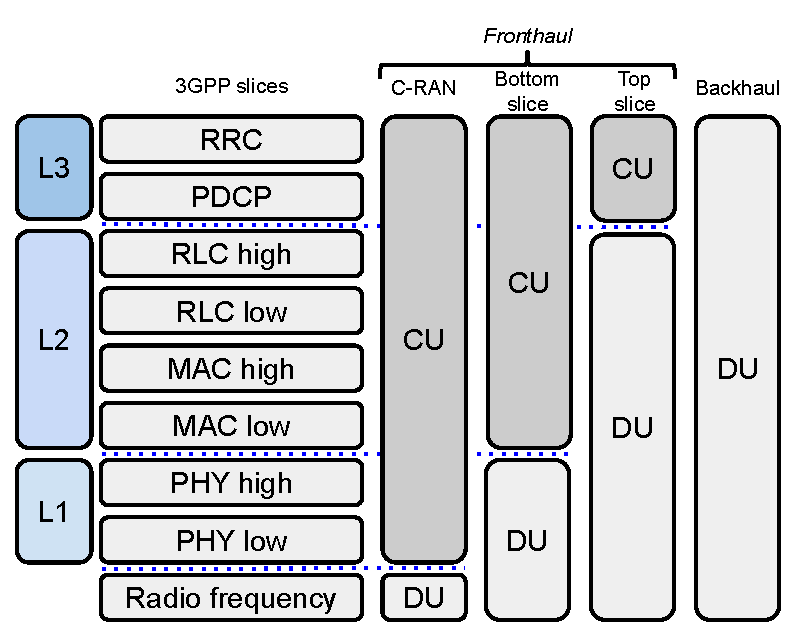
\includegraphics[width=0.45\textwidth]{figs/splits_layers.pdf}
  \end{center}
\caption{Division of functions between the central and the distributed units.}
\label{fig:splitsLayers}
\end{figure}

It is important to note that this new flexible architecture of RAN composed of distributed data units (DU/gNB-DU) and control (CU/gNB-CU) brought changes to the transport network between the access and the core of the 5G system. Currently, the transport network is being redesigned and developed considering segments of fronthaul, midhaul, and backhaul. The fronthaul is responsible for the communication between RRH/vRRH and DU/gNB-DU. In the midhaul segment, communication takes place between DU/gNB-DU and CU/gNB-CU. Finally, the backhaul performs the communication between CU/gNB-CU and the new core of the 5G system. Additionally, approaches are expected to adopt the integration between transport segments, in a configuration of crosshaul~\cite {Gonzalez-Diaz:19,fonseca-sbrc-2019}, in which the objective is to explore the efficient use of resources high-cost transportation. Orchestrating the workloads of vRANs in this new architecture is a subject of considerable research today.

\subsection{RAN demonstration} \label{subsec:demo_RAN}

\subsection*{Goals}

One objective of the demonstration is to present practically the functionalities of a RAN, using open software and hardware. Another goal is to briefly comment on the software installation and configuration processes that implement the RAN, making available material for replication of this demonstration.

\begin{figure*}[htb] 
 \begin{center}
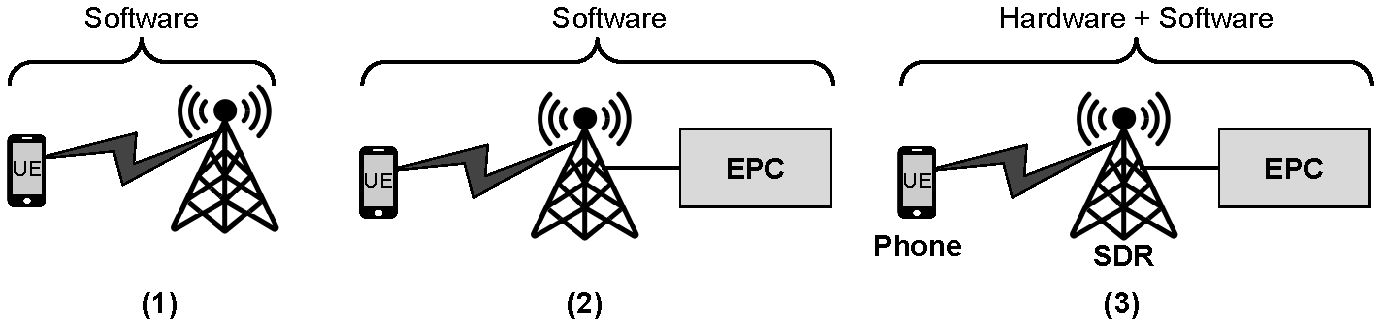
\includegraphics[width=0.9\textwidth]{figs/demo1-en.pdf}
  \end{center}
\caption{Experiments with a softwarized RAN.}
\label{fig:demo1}
\end{figure*}

\subsection*{Description}

In this demonstration, we create an operational eNodeB, \textit{i.e.}, the main element of a RAN, based on LTE technology and using open-source software. In addition to the RAN, the software is also capable of emulating functional UEs. The demonstration is organized in 3 experiments: (1) UE and RAN emulated by software, without the core; (2) UE, RAN and EPC core, all implemented in software; and (3) UE in hardware (conventional cell phone), RAN in hardware (SDR - Software-Defined Radio) and software, and EPC core implemented in software. All components are implemented using Docker containers that can be hosted on a cloud infrastructure. Fig.~\ref{fig:demo1} shows the software and hardware components that are used in the RAN demo.

\subsection*{Additional information}

During the tutorial, demonstration videos of the experiments are presented. Furthermore, manuals are available with details on how the tests can be replicated. Finally, the containers and any extra code produced by the authors needed to replicate the experiments are also publicly available.

The repository of this tutorial:\\
\url{https://github.com/LABORA-INF-UFG/NetSoft2020-Tutorial4}.